\documentclass[11pt]{article}

% ---------- Packages ----------
\usepackage[margin=1in]{geometry}
\usepackage[parfill]{parskip}
\usepackage{amsmath, amssymb}
\setcounter{MaxMatrixCols}{20}
\usepackage{booktabs}
\usepackage{array}
\usepackage{xcolor}
\usepackage{colortbl}
\usepackage{tikz}
\usepackage{float}
\usepackage[hidelinks]{hyperref}

% ---------- Title & Authors ----------
\title{\textbf{MA 232 Course Project 2:}\\ How AI Detects Objects: A Linear Algebra Approach to Pattern Recognition}
\author{Derrick Sual \and Ryan Kropac \and Mahanth Chintha}
\date{\today}

\begin{document}
\maketitle

\begin{center}
\textit{“I pledge my honor that I have abided by the Stevens Honor System.”}
\end{center}

\vspace{1em}

% ===========================================================================
\section*{Part A: Convert the Pattern into a Vector}
% Assigned to: Derrick Sual
% ===========================================================================

% --- Task A.1: Convert the given grid into a vector w in R^16 ---
\subsubsection*{Task A.1: Target Grid and Vector Representation}
\textit{Convert the given grid into a vector $w \in \mathbb{R}^{16}$.}

\vspace{0.4em}
\textbf{Answer:}
The target pattern is a $4 \times 4$ binary grid with blue cells as $1$ and white cells as $0$:

\begin{center}
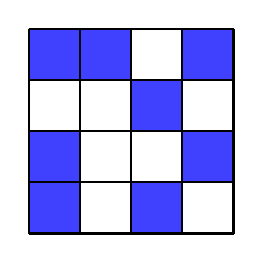
\begin{tikzpicture}[scale=0.65]
  % Grid base
  \draw[step=1cm, black, thick] (0, 0) grid (4, 4);
  % Fill the 8 blue cells
  % Row 1 (top): cells at cols 0, 1, 3
  \fill[blue!75] (0, 3) rectangle (1, 4);
  \fill[blue!75] (1, 3) rectangle (2, 4);
  \fill[blue!75] (3, 3) rectangle (4, 4);
  % Row 2: cell at col 2
  \fill[blue!75] (2, 2) rectangle (3, 3);
  % Row 3: cells at cols 0, 3
  \fill[blue!75] (0, 1) rectangle (1, 2);
  \fill[blue!75] (3, 1) rectangle (4, 2);
  % Row 4 (bottom): cells at cols 0, 2
  \fill[blue!75] (0, 0) rectangle (1, 1);
  \fill[blue!75] (2, 0) rectangle (3, 1);
  % Redraw outlines on top
  \draw[step=1cm, black, thick] (0, 0) grid (4, 4);
\end{tikzpicture}
\end{center}

Reading row by row from top to bottom (left to right) yields the target vector $w \in \mathbb{R}^{16}$:
\[
w = \begin{bmatrix}
1 & 1 & 0 & 1 & 0 & 0 & 1 & 0 & 1 & 0 & 0 & 1 & 1 & 0 & 1 & 0
\end{bmatrix}^T
\]

\vspace{0.8em}

% --- Task A.2: Blue and white cell count ---
\subsubsection*{Task A.2: Cell Counts}
\textit{How many blue cells and white cells does the target pattern contain?}

\vspace{0.4em}
\textbf{Answer:}
The target pattern contains \textbf{8 blue cells} (value 1) and \textbf{8 white cells} (value 0), for a total of 16 cells.

\vspace{0.5em}

% --- Task A.3: Arbitrary blue-and-white grid representation ---
\subsubsection*{Task A.3: General Pattern Encoding Procedure}
\textit{Explain how an arbitrary blue-and-white $4 \times 4$ grid can be represented by a vector $u \in \{0, 1\}^{16}$.}

\vspace{0.4em}
\textbf{Answer:}
We can treat the $4 \times 4$ grid like a coordinate system where each cell has a row $i$ and column $j$ (from 1 to 4). Each cell takes a value of $1$ if it is filled with blue, or $0$ if it is white.

To flatten this into a vector, we read the grid row by row from top to bottom (left to right) into a 16-element column vector $u \in \{0, 1\}^{16}$. Because there are 16 cells and each cell can be either 0 or 1, this vector representation accounts for all $2^{16} = 65,536$ possible blue-and-white patterns.

\vspace{1.5em}

% ===========================================================================
\section*{Part B: Construct a Matrix for Pattern Recognition}
% Assigned to: Derrick Sual
% ===========================================================================

% --- Task B.1: Information represented by vector u ---
\subsubsection*{Task B.1: Information Represented by Vector $u$}
\textit{Explain what information is represented by the vector $u$.}

\vspace{0.4em}
\textbf{Answer:}
The vector $u \in \{0, 1\}^{16}$ represents any $4 \times 4$ test pattern we want to check against our target pattern. Each of the 16 entries in $u$ tells us whether that specific box on the grid is blue ($1$) or white ($0$).

\vspace{0.8em}

% --- Task B.2: Role of quadratic form ---
\subsubsection*{Task B.2: Role of Quadratic Form $Q(u) = u^T M u$}
\textit{Describe the role of the quadratic form $Q(u) = u^T M u$ in recognizing a pattern.}

\vspace{0.4em}
\textbf{Answer:}
The quadratic form $Q(u) = u^T M u$ works like a scoring function for any test pattern $u$:
\begin{itemize}
    \item If the function returns $0$, the test pattern matches our target pattern ($Q(w) = w^T M w = 0$).
    \item If the function returns a nonzero (positive) score, the pattern is not the target pattern ($Q(u) \neq 0$).
\end{itemize}
This turns pattern recognition into a simple check: an input pattern is recognized as the target pattern if and only if $Q(u) = 0$.

\vspace{0.5em}

% --- Task B.3: Construct 16x16 matrix M ---
\subsubsection*{Task B.3: Construction of Matrix $M$}
\textit{Construct a $16 \times 16$ matrix $M$ that satisfies the two conditions: $w^T M w = 0$ and $u^T M u \neq 0$ for every other nonzero binary vector $u \neq w$.}

\vspace{0.4em}
\textbf{Answer:}
We construct $M$ in the form $M = B^T B$. To guarantee that $M w = \mathbf{0}$, we choose the rows of $B$ to be 15 vectors $v_1, \dots, v_{15}$ that are all perpendicular (orthogonal) to $w$.

\begin{enumerate}
    \item Setting the dot product $w \cdot v = 0$ using our target vector gives:
    \[
    v_1 + v_2 + v_4 + v_7 + v_9 + v_{12} + v_{13} + v_{15} = 0
    \]
    \item Solving for the first component:
    \[
    v_1 = -(v_2 + v_4 + v_7 + v_9 + v_{12} + v_{13} + v_{15})
    \]
    Setting each of the other 15 free components to 1 (one at a time, with all others 0) produces a basis of 15 vectors $\{v_1, v_2, \dots, v_{15}\}$ that are all orthogonal to $w$.
    \item We stack these 15 vectors as rows of a $15 \times 16$ matrix $B$:
    \[
    B = \begin{bmatrix} v_1^T \\ v_2^T \\ \vdots \\ v_{15}^T \end{bmatrix}
    \]
    \item We set $M = B^T B$, which produces our $16 \times 16$ matrix.
\end{enumerate}

\vspace{0.8em}

% --- Task B.4: Show w^T M w = 0 ---
\subsubsection*{Task B.4: Verification of the Null Target Condition}
\textit{Show that your matrix satisfies $w^T M w = 0$.}

\vspace{0.4em}
\textbf{Answer:}
Because every row of $B$ was chosen to be orthogonal to $w$, multiplying $B$ by $w$ gives:
\[
B w = \begin{bmatrix} v_1^T w \\ \vdots \\ v_{15}^T w \end{bmatrix} = \begin{bmatrix} 0 \\ \vdots \\ 0 \end{bmatrix} = \mathbf{0}
\]
This means $M w = B^T (B w) = B^T \mathbf{0} = \mathbf{0}$.

Evaluating the quadratic form for the target vector gives:
\[
w^T M w = w^T (M w) = w^T \mathbf{0} = 0
\]

\vspace{0.8em}

% --- Task B.5: Explain why Q(u) != 0 for all other nonzero binary vectors ---
\subsubsection*{Task B.5: Nonzero Condition for Non-Target Binary Vectors}
\textit{Explain why the quadratic form must be nonzero for every other nonzero binary vector.}

\vspace{0.4em}
\textbf{Answer:}
Using the transpose product rule, the quadratic form can be written as:
\[
u^T M u = u^T (B^T B) u = (B u)^T (B u) = \|B u\|^2
\]
Because $\|B u\|^2$ is a squared length, it is always $\ge 0$, and equals 0 if and only if $B u = \mathbf{0}$. The only vectors satisfying $B u = \mathbf{0}$ are scalar multiples of the target pattern, $u = c \cdot w$.

Since $u$ is restricted to binary patterns ($0$ and $1$ only):
\begin{itemize}
    \item $c = 0 \implies u = \mathbf{0}$ (the all-white grid).
    \item $c = 1 \implies u = w$ (the target pattern).
\end{itemize}
For any other nonzero binary vector $u \neq w$, $u$ is not a multiple of $w$, which means $B u \neq \mathbf{0}$. This guarantees that the score is strictly positive:
\[
u^T M u = \|B u\|^2 > 0 \neq 0
\]

\vspace{0.8em}

% --- Task B.6: Symmetry and Invertibility ---
\subsubsection*{Task B.6: Symmetry and Invertibility of $M$}
\textit{State whether your matrix is symmetric and whether it is invertible. Justify your answers.}

\vspace{0.4em}
\textbf{Answer:}
\begin{itemize}
    \item \textbf{Symmetry: Yes.} Using the transpose product rule:
    \[
    M^T = (B^T B)^T = B^T (B^T)^T = B^T B = M
    \]
    Since $M^T = M$, matrix $M$ is symmetric.
    \item \textbf{Invertibility: No.} From Task B.4, we know that $M w = \mathbf{0}$. Because matrix $M$ maps a nonzero vector ($w \neq \mathbf{0}$) to the zero vector, $w$ is a non-trivial vector in the nullspace of $M$. Therefore, $\det(M) = 0$, its rank is 15 (not full rank 16), and $M$ is not invertible.
\end{itemize}

\newpage

% ===========================================================================
\section*{Part C: Verify the Recognition Rule}
% Assigned to: Member 2 (Ryan Kropac)
% ===========================================================================

% --- Task C.1: Systematic verification method ---
\subsubsection*{Task C.1: Systematic Verification Methodology}
\textit{Develop a systematic method to verify your matrix.}

\vspace{0.4em}
\textbf{Answer:} To verify our matrix \(M\), we first check that the target pattern produces \(Q(w)=0\). We then test other patterns to make sure they produce nonzero values. Finally, we use Python to check all 65,535 possible nonzero binary patterns and confirm that only the target produces zero.

\vspace{0.5em}

% --- Task C.2: Target vector verification ---
\subsubsection*{Task C.2: Verification of the Target Vector}
\textit{Verify the quadratic-form value for the target vector.}

\vspace{0.4em}
\textbf{Answer:} To verify that the target pattern produces zero, we use the matrix constructed in Part B, where \(M=B^TB\).
Substituting this into the quadratic form gives:
\[
Q(w)=w^TMw=w^TB^TBw
\]
We can rewrite this as:
\[
Q(w)=(Bw)^T(Bw)
\]
Since \(B\) was constructed so that \(Bw=0\), we get:
\[
Q(w)=0^T0=0
\]
Therefore, the target vector satisfies the recognition condition \(w^TMw=0\).

\vspace{0.5em}

% --- Task C.3: Testing required sample patterns ---
\subsubsection*{Task C.3: Testing on Required Binary Patterns}
\textit{Test your matrix on several other binary patterns, including: a grid with only one blue cell, a grid with two blue cells, a grid with three blue cells in different positions, and the grid with all 16 cells blue.}

\vspace{0.4em}
\textbf{Answer:} 
We tested our matrix $M$ using several different binary patterns and calculated $Q(u)=u^TMu$ for each.
\begin{center}
\begin{tabular}{|l|c|}
\hline
Test Pattern & $Q(u)$ \\
\hline
One blue cell (Cell 1) & 7 \\
One blue cell (Cell 3) & 1 \\
Two blue cells (Cells 1, 2) & 6 \\
Two blue cells (Cells 1, 3) & 8 \\
Three blue cells (Cells 1, 2, 4) & 5 \\
Three blue cells (Cells 3, 5, 6) & 3 \\
All 16 cells blue & 8 \\
\hline
\end{tabular}
\end{center}
All tested patterns produced nonzero values. This confirms that our matrix correctly rejects these patterns because none matches the target vector $w$.

\vspace{0.5em}

% --- Task C.4: Explaining verification over all 65,535 vectors ---
\subsubsection*{Task C.4: Exhaustive Verification of All $2^{16} - 1 = 65,535$ Nonzero Binary Vectors}
\textit{Explain how you can verify the condition for all $2^{16} - 1 = 65,535$ nonzero binary vectors.}

\vspace{0.4em}
\textbf{Answer:} 
There are $2^{16} = 65,536$ possible binary vectors for a $4 \times 4$ grid. Excluding the all-zero vector leaves 65,535 nonzero patterns.

We can use Python to generate every possible binary vector and calculate $Q(u) = u^T M u$ for each one. We then check that the target vector $w$ is the only nonzero vector that produces zero.

This method allows us to verify every possible pattern rather than relying only on a few examples.

\vspace{0.5em}

% --- Task C.5: Table of 10 test patterns ---
\subsubsection*{Task C.5: Table of Test Patterns and Values}
\textit{Present a table of at least 10 test patterns, their binary vectors, and the corresponding quadratic-form values.}

Table~\ref{tab:sample_patterns} presents the quadratic-form values calculated using matrix $M$ for 10 different binary patterns.


\begin{table}[H]
\centering
\scriptsize
\begin{tabular}{clcc}
\toprule
\# & Test Pattern & Binary Vector & $Q(u)$ \\
\midrule
1 & Target & 1101001010011010 & 0 \\
2 & Cell 1 & 1000000000000000 & 7 \\
3 & Cell 3 & 0010000000000000 & 1 \\
4 & Cells 1, 2 & 1100000000000000 & 6 \\
5 & Cells 1, 3 & 1010000000000000 & 8 \\
6 & Cells 1, 2, 4 & 1101000000000000 & 5 \\
7 & Cells 3, 5, 6 & 0010110000000000 & 3 \\
8 & Cells 1, 2, 4, 7 & 1101001000000000 & 4 \\
9 & Inverted target & 0010110101100101 & 8 \\
10 & All blue & 1111111111111111 & 8 \\
\bottomrule
\end{tabular}
\caption{Test patterns and quadratic-form values.}
\label{tab:sample_patterns}
\end{table}

\vspace{0.5em}

% --- Task C.6: Proving all nonzero binary patterns are satisfied ---
\subsubsection*{Task C.6: Generality Beyond the Sample Table}
\textit{State how you know that your construction satisfies the requirement for all nonzero binary patterns, not merely the patterns in your sample table.}

\vspace{0.4em}
\textbf{Answer:} 
Our matrix $M$ was constructed as $M = B^TB$, where the null space of $B$ is spanned by the target vector $w$.

Therefore, $Q(u) = u^TMu = (Bu)^T(Bu) = 0$ only when $u$ is a multiple of $w$.

Since we are only considering binary vectors, the only possible multiples are the zero vector and $w$ itself. The zero vector is excluded from the requirements.

Therefore, $w$ is the only nonzero binary vector that produces zero, proving that our matrix works for all 65,535 nonzero patterns.

\newpage

% ===========================================================================
\section*{Part D: Explore Different Matrix Constructions}
% Assigned to: Member 2 (Ryan Kropac)
% ===========================================================================

\subsection*{D.1: Construct a Second Matrix}

% --- Task D.1.a: Find second matrix N ---
\subsubsection*{Task D.1.a: Construction of Second Matrix $N$}
\textit{Find a second $16 \times 16$ matrix $N$, different from your original matrix $M$, that recognizes the same target pattern.}

\vspace{0.4em}
\textbf{Answer:} 
We construct a second matrix $N$ using the formula

\[
N = 8I - ww^T
\]

where $I$ is the $16 \times 16$ identity matrix and
$w$ is our target vector.

Since $w$ contains eight ones, $w^Tw = 8$.
This gives us a different matrix from $M$ that
recognizes the same target pattern.

\begin{center}
\resizebox{\textwidth}{!}{$
N = \begin{bmatrix}
7&-1&0&-1&0&0&-1&0&-1&0&0&-1&-1&0&-1&0\\
-1&7&0&-1&0&0&-1&0&-1&0&0&-1&-1&0&-1&0\\
0&0&8&0&0&0&0&0&0&0&0&0&0&0&0&0\\
-1&-1&0&7&0&0&-1&0&-1&0&0&-1&-1&0&-1&0\\
0&0&0&0&8&0&0&0&0&0&0&0&0&0&0&0\\
0&0&0&0&0&8&0&0&0&0&0&0&0&0&0&0\\
-1&-1&0&-1&0&0&7&0&-1&0&0&-1&-1&0&-1&0\\
0&0&0&0&0&0&0&8&0&0&0&0&0&0&0&0\\
-1&-1&0&-1&0&0&-1&0&7&0&0&-1&-1&0&-1&0\\
0&0&0&0&0&0&0&0&0&8&0&0&0&0&0&0\\
0&0&0&0&0&0&0&0&0&0&8&0&0&0&0&0\\
-1&-1&0&-1&0&0&-1&0&-1&0&0&7&-1&0&-1&0\\
-1&-1&0&-1&0&0&-1&0&-1&0&0&-1&7&0&-1&0\\
0&0&0&0&0&0&0&0&0&0&0&0&0&8&0&0\\
-1&-1&0&-1&0&0&-1&0&-1&0&0&-1&-1&0&7&0\\
0&0&0&0&0&0&0&0&0&0&0&0&0&0&0&8
\end{bmatrix}
$}
\end{center}

\newpage

% --- Task D.1.b: Verify recognition conditions for N ---
\subsubsection*{Task D.1.b: Verification of Conditions for Matrix $N$}
\textit{Verify that $w^T N w = 0$ and $u^T N u \neq 0$ for every other nonzero binary vector $u \neq w$.}

\vspace{0.4em}
\textbf{Answer:} 
To verify that $N$ recognizes the target, we calculate:

\[
w^TNw = w^T(8I - ww^T)w
\]

\[
= 8(w^Tw) - (w^Tw)^2
\]

\[
= 8(8) - 8^2 = 64 - 64 = 0
\]

For any vector $u$, we have:

\[
u^TNu = 8\|u\|^2 - (w^Tu)^2
\]

By the Cauchy-Schwarz inequality,

\[
(w^Tu)^2 \leq 8\|u\|^2
\]

Equality occurs only when $u$ is a multiple of $w$.
Since $u$ is binary, the only possibilities are
$u = 0$ and $u = w$.

Therefore, every other nonzero binary vector
produces a positive value, so $N$ satisfies
the recognition conditions.

\vspace{0.5em}

% --- Task D.1.c: Comparison between M and N ---
\subsubsection*{Task D.1.c: Comparison Between Matrices $M$ and $N$}
\textit{Explain how the second matrix differs from the first and why both matrices work.}

\vspace{0.4em}
\textbf{Answer:} 
Our original matrix $M = B^TB$ was constructed
using vectors perpendicular to the target $w$.

Our second matrix $N = 8I - ww^T$ was constructed
using an orthogonal projection method.

Although the matrices contain different values,
both produce zero for the target pattern and
positive values for every other nonzero binary
pattern.

Therefore, both matrices successfully recognize
the same target.

\vspace{1em}

\subsection*{D.2: Investigate Matrix Structure}

% --- Task D.2.a: Can matrix with off-diagonal entries work? ---
\subsubsection*{Task D.2.a: Viability of Off-Diagonal Entries}
\textit{Can a matrix with nonzero off-diagonal entries satisfy the requirements?}

\vspace{0.4em}
\textbf{Answer:} 
Yes, a matrix with nonzero off-diagonal entries
can satisfy the recognition conditions.

In fact, both of our matrices $M$ and $N$ contain
nonzero off-diagonal entries and successfully
recognize the target pattern.

\vspace{0.5em}

% --- Task D.2.b: Contribution of matrix entries to u^T M u ---
\subsubsection*{Task D.2.b: Contribution of Matrix Entries to $u^T M u$}
\textit{Explain how the entries of a matrix contribute to the value of $u^T M u$.}

\vspace{0.4em}
\textbf{Answer:} 
The quadratic form can be written as:

\[
u^TMu = \sum_{i=1}^{16}\sum_{j=1}^{16}
M_{ij}u_i u_j
\]

Diagonal entries contribute terms involving
the square of a single element, while
off-diagonal entries contribute terms involving
two different elements.

For binary vectors, each element is either
0 or 1. Therefore, off-diagonal terms contribute
only when both corresponding cells are blue.

\vspace{0.5em}

% --- Task D.2.c: Construct or describe non-diagonal matrix ---
\subsubsection*{Task D.2.c: Construction/Description of Non-Diagonal Matrix}
\textit{Construct or describe a non-diagonal matrix that satisfies the recognition condition, if possible.}

\vspace{0.4em}
\textbf{Answer:} 
Our second matrix $N = 8I - ww^T$ is an example
of a non-diagonal matrix that satisfies the
recognition conditions.

Its entries are defined by:

\[
N_{ij} =
\begin{cases}
7 & \text{if } i=j \text{ and } w_i=1,\\
8 & \text{if } i=j \text{ and } w_i=0,\\
-1 & \text{if } i\neq j \text{ and } w_i=w_j=1,\\
0 & \text{otherwise}.
\end{cases}
\]

Since $N$ contains off-diagonal entries equal
to $-1$, it is not diagonal.

As shown in D.1(b), this matrix produces zero
only for the target vector and the excluded
zero vector. Therefore, a matrix does not need
to be diagonal to recognize the target pattern.

\newpage

% ===========================================================================
\section*{Part E: Reflection and Applications}
% Assigned to: Group Collaboration (Led by Mahanth Chintha)
% ===========================================================================

\textit{Write a single cohesive reflection of approximately 300--500 words in continuous prose addressing the following topics (do not answer them as separate numbered questions):}
\begin{itemize}
    \item How converting a visual grid into a vector makes mathematical analysis possible.
    \item The challenges faced in constructing the recognition matrix.
    \item How pattern uniqueness was verified mathematically and computationally.
    \item Why systematic verification is critical in pattern recognition.
    \item Real-world applications of this approach (e.g., image processing, computer vision, data science).
\end{itemize}

\vspace{0.8em}

This project asked us to teach a computer to recognize a pattern using linear algebra. We began by converting a $4\times4$ grid of blue and white squares into a vector. We created this vector by reading the grid row by row and representing each blue cell as $1$ and each white cell as $0$. By doing so, we created a vector in $\mathbb{R}^{16}$. This allowed us to use matrices and dot products to determine whether a test pattern matched our target pattern. We also found that there are $2^{16}=65{,}536$ possible patterns that could all be analyzed using a similar approach.

The hardest part of this project was constructing the recognition matrix. We needed a matrix $M$ such that $w^TMw=0$ for our target pattern, while producing a positive value for all other nonzero binary vectors. Although we initially struggled to satisfy both conditions at once, we came to a conclusion. Our solution was to construct $M=B^TB$, where the rows of $B$ are perpendicular to $w$. This ensures that $Bw=0$, and it also transforms the quadratic form into $\|Bu\|^2$. This guarantees a nonnegative value since a squared length can never be negative. This approach also helped us prove that the target was unique. Since $Q(u)=0$ only when $Bu=0$, $u$ must be a multiple of $w$. Because our vectors contain only $0$s and $1$s, the only possibilities are the zero vector and our target $w$.

In order to verify our results, we tested multiple patterns. These patterns included the single blue cells, the inverted target, and the all-blue grid. We also wrote a Python program to check all $65{,}535$ nonzero binary patterns. Additionally, we constructed a second recognition matrix, $N=8I-ww^T$. This demonstrated that multiple matrices can satisfy the same requirements. One important lesson we learned was that testing a few examples does not automatically prove a method works. A matrix might pass ten tests but fail on the eleventh. As a result, we combined mathematical proofs with computational verification, giving us greater confidence in our results.

This project also showed us how linear algebra can be applied to pattern recognition. In real systems, incorrectly identifying or missing a pattern could lead to serious problems, making accuracy and precision essential. Similar pattern recognition concepts appear in real-world applications such as image processing, computer vision, and data science, where images and other information are converted into vectors and compared against known patterns.

Although our $4\times4$ grid was a simplified example, it demonstrated the same fundamental idea: representing visual information mathematically allows individuals to use matrices to recognize patterns reliably.


\vspace{1.5em}

% ===========================================================================
% Note on Part F: Group Performance Evaluation
% Per project instructions, Part F is an entirely confidential individual 
% evaluation submitted independently by each group member. It is omitted 
% from this joint technical report.
% ===========================================================================

\end{document}
